\section{Soft drop in future collider performance}
In this section, we use the specific method, soft-drop, to study the performance of the detector with the different detector cell sizes and center-of-mass(c.m.) energies. 
\subsection{The technic of Soft-drop}
Soft-drop(SD)[\ref{}], taking literally, is the technique that reserves the soft $P_{T}$ of jets which is greater than the set threshold. The formula and the technique are as following:
\begin{equation} \label{eq:soft-drop}
\frac{min(P_{T1},P_{T2})}{P_{T1}+P_{T2}}>Z_{cut}(\frac{\Delta R_{12}}{R_{0}})^{\beta}
\end{equation}
$P_{T1}$,$P_{T2}$ are $P_{T}$ of the two jets. $Z_{cut}$ is soft drop threshold. $\Delta R_{12}$ are the two jets distance on the $\eta$-$\phi$ plane. $\beta$ is the angular exponent. $R_{0}$ is the characteristic radius with clustering.
\begin{enumerate}
\item First, Anti-kt(AK) algorithm is used to reconstruct jets.
\item Second, after reconstructing the AK4 jets, Cambridge-Aachen (C/A) algorithm is used to decluster the jets into two (C/A) jets.
\item Third, these two jets are compared with the formula \ref{eq:soft-drop}. Two jets will be reserved when they pass the formula, otherwise, the softer jet of two jets will be removed.
\item Finally, loop the procedure from 1.to 3.until the jets can not be declusteded into two jets.
\end{enumerate}
In our study, we compare $\beta=0$ with $\beta=2$ and observe their performance in the future detector. For $\beta=0$, the selection only depends on the $Z_{cut}$. For $\beta=2$, the selection depends on the angle of two declustering jets and $Z_{cut}$, it is infrared and collinear (IRC) safe. The paper of SD[\ref{}] refer to the detail of it.   
\subsection{Analysis method}
First, start at the central value of the signal median bin's right boundary. Then, add the left and right bins symmetrically to extend the width and draw the Receiver Operating Characteristic(ROC) curves.
%The width is extended from the central bin which is right boundary of the median bin, then draw the Receiver Operating Characteristic(ROC) curves with the left and right bin.
\subsection{The results and conclusions}
In the Figure[\ref{fig:cluster_mass_mmdt_ww}][\ref{fig:cluster_mass_mmdt_tt}][\ref{fig:cluster_mass_sdb2_ww}][\ref{fig:cluster_mass_sdb2_tt}], distributions of mass under SD at  $\beta=0$ and $\beta=2$ with different c.m. energies and detector cell sizes are presented. Because different $\beta$ and signal contain the different ranges of mass, we choose the different ranges in the histograms.\\

In the Figure [\ref{fig:cluster_mass_mmdt_ww_ROC}][\ref{fig:cluster_mass_mmdt_tt_ROC}][\ref{fig:cluster_mass_sdb2_ww_ROC}][\ref{fig:cluster_mass_sdb2_tt_ROC}], ROC curves are used to perform the study of comparing different parameters. The figures want to show which detector cell size has the best "background rejection" with different c.m. energies. In other words, which cell size has the best separation power to distinguish signal from background with different c.m. energies.\\

In the Figure [\ref{fig:cluster_mass_mmdt_ww_ROC}], they show the ROC curves for WW signal at SD with $\beta=0$  with different detector cell sizes and c.m. energies. These performances show that 5,10, 20 TeV have the best distinguish power with the smallest (1$\times$1) detector cell sizes. Similar to the tt signal at same $\beta$ in Figure[\ref{fig:cluster_mass_mmdt_tt_ROC}], they have the best distinguish power at 10, 20 TeV with the smallest (1$\times$1) detector cell sizes.\\

Oppositely, in the figure [\ref{fig:cluster_mass_sdb2_ww_ROC}] and figure [\ref{fig:cluster_mass_sdb2_tt_ROC}], these show the ROC curves for WW and tt signal at SD with $\beta=2$. They show the same conclusions that all c.m. energies don't have any improvements with the smallest (1$\times$1) detector cell sizes. Some of the ROC curves with the different detector cell sizes almost overlap, that means the performances of this three sizes are very similar. In addition, some of them have the best distinguish power with the bigger detector (5$\times$5 or 20$\times$20) cell size. \\

After this study, we find that SD with $\beta=0$ has the better performance for distinguishing signal from background than $\beta=2$. so we choose SD at $\beta=0$ to be our mass cut and apply it in other jet substructure variables for the next step.\\
 
%50bins
\begin{figure}
\begin{center}
   \subfigure[5TeV at 20$\times$20(cm$\times$cm) with cluster] {
   \includegraphics[width=0.22\textwidth]{figs/Dis_cluster_010_mass_mmdt_5tev_04_no_UOF.eps}
   }
      \subfigure[10TeV at 20$\times$20(cm$\times$cm) with cluster] {
   \includegraphics[width=0.22\textwidth]{figs/Dis_cluster_010_mass_mmdt_10tev_04_no_UOF.eps}
   }
   \subfigure[20TeV at 20$\times$20(cm$\times$cm) with cluster] {
   \includegraphics[width=0.22\textwidth]{figs/Dis_cluster_010_mass_mmdt_20tev_04_no_UOF.eps}
   }
    \subfigure[40TeV at 20$\times$20(cm$\times$cm) with cluster] {
   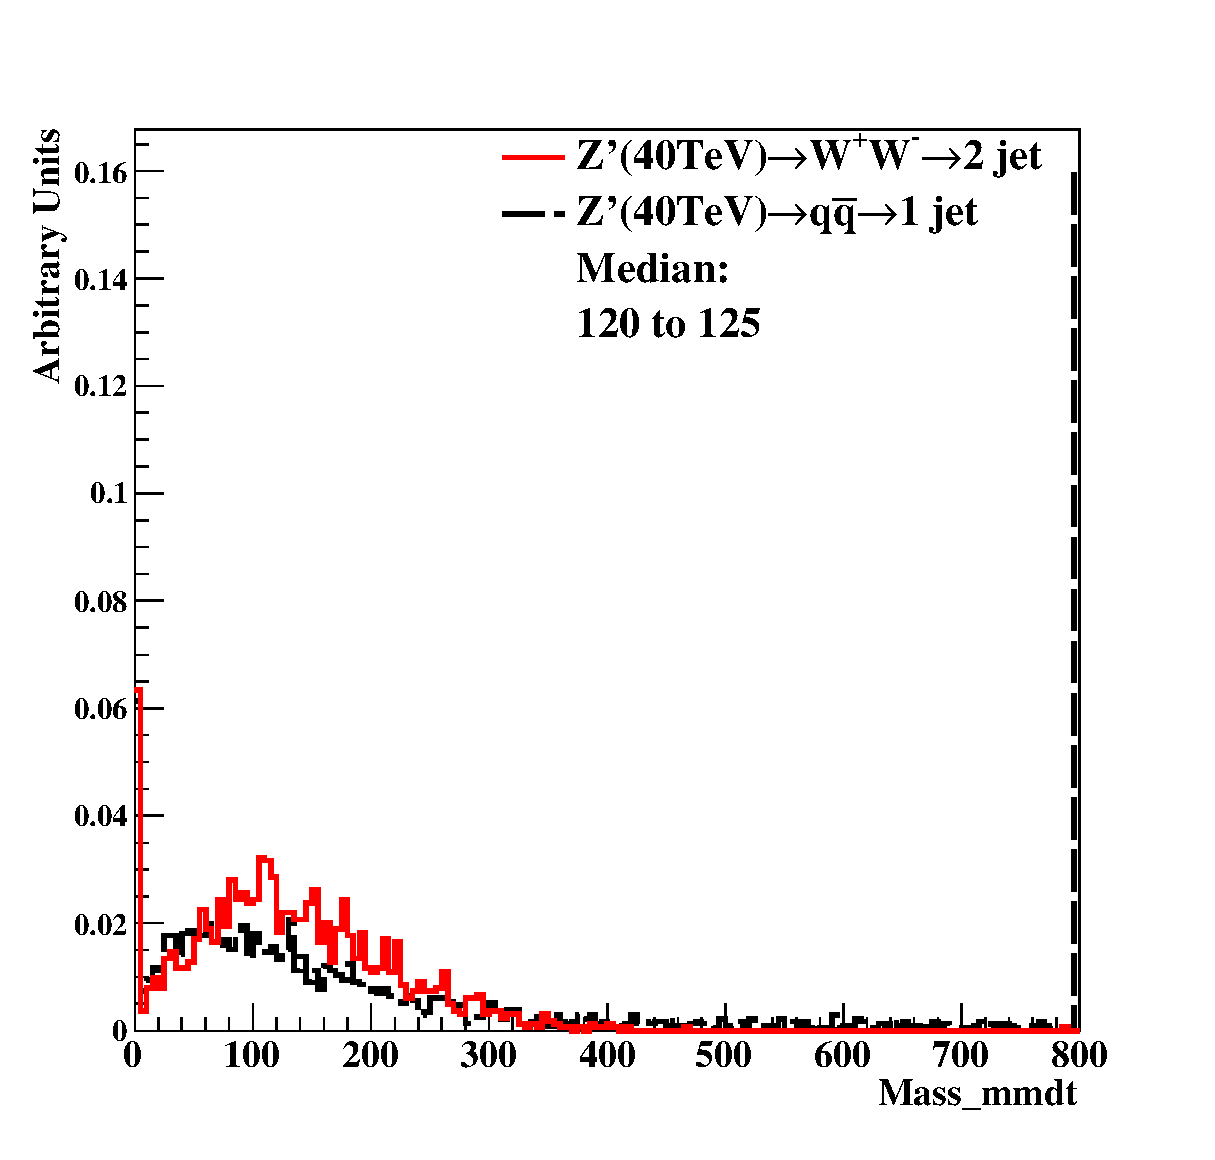
\includegraphics[width=0.22\textwidth]{figs/Dis_cluster_010_mass_mmdt_40tev_04_no_UOF.eps}
   }
   \subfigure[5TeV at 5$\times$5(cm$\times$cm) with cluster] {
   \includegraphics[width=0.22\textwidth]{figs/Dis_cluster_009_mass_mmdt_5tev_04_no_UOF.eps}
   }
   \subfigure[10TeV at 5$\times$5(cm$\times$cm) with cluster] {
   \includegraphics[width=0.22\textwidth]{figs/Dis_cluster_009_mass_mmdt_10tev_04_no_UOF.eps}
   }
      \subfigure[20TeV at 5$\times$5(cm$\times$cm) with cluster] {
   \includegraphics[width=0.22\textwidth]{figs/Dis_cluster_009_mass_mmdt_20tev_04_no_UOF.eps}\hfill
   }
      \subfigure[40TeV at 5$\times$5(cm$\times$cm) with cluster] {
   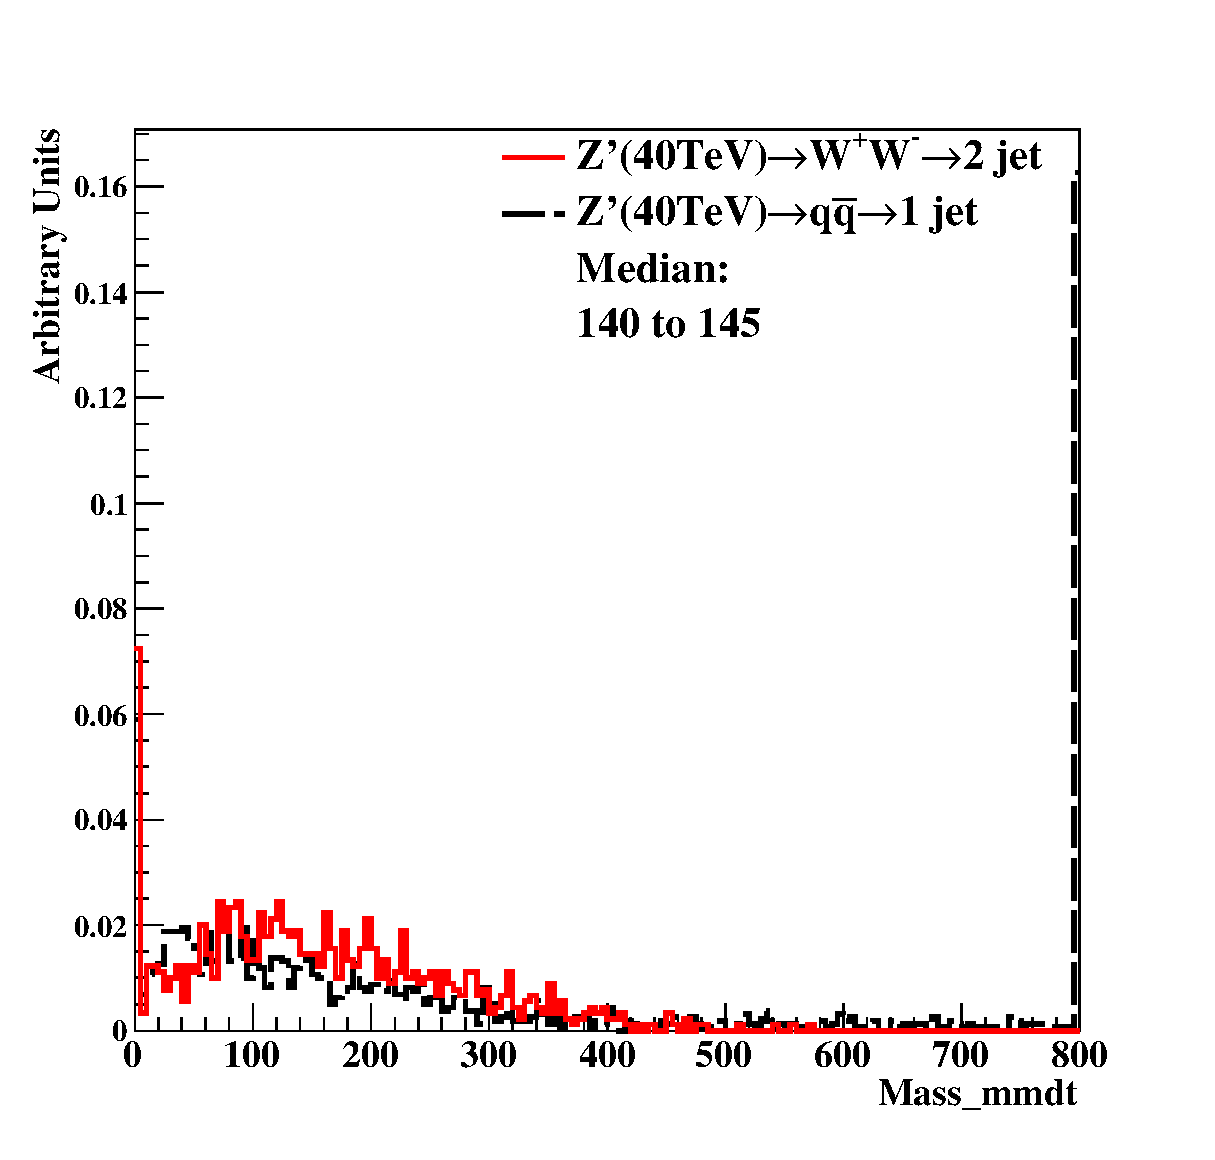
\includegraphics[width=0.22\textwidth]{figs/Dis_cluster_009_mass_mmdt_40tev_04_no_UOF.eps}\hfill
   }
   \subfigure[5TeV at 1$\times$1(cm$\times$cm) with cluster] {
   \includegraphics[width=0.22\textwidth]{figs/Dis_cluster_012_mass_mmdt_5tev_04_no_UOF.eps}\hfill
   }
    \subfigure[10TeV at 1$\times$1(cm$\times$cm) with cluster] {
   \includegraphics[width=0.22\textwidth]{figs/Dis_cluster_012_mass_mmdt_10tev_04_no_UOF.eps}
   }
   \subfigure[20TeV at 1$\times$1(cm$\times$cm) with cluster] {
   \includegraphics[width=0.22\textwidth]{figs/Dis_cluster_012_mass_mmdt_20tev_04_no_UOF.eps}\hfill
   }
      \subfigure[40TeV at 1$\times$1(cm$\times$cm) with cluster] {
   \includegraphics[width=0.22\textwidth]{figs/Dis_cluster_012_mass_mmdt_40tev_04_no_UOF.eps}
   }

\end{center}
\caption{Distributions of mass soft drop at $\beta$=0, signal=ww, with 5,10,20,40TeV c.m. energy and different detector sizes. Cell Size in 20$\times$20, 5$\times$5, and 1$\times$1(cm$\times$cm) are shown here.}
\label{fig:cluster_mass_mmdt_ww}
\end{figure}


\begin{figure}
\begin{center}
  \subfigure[Central at Median($20\times20$=,$5\times5$=,$1\times1$=) change width with cluster at 5TeV] {
  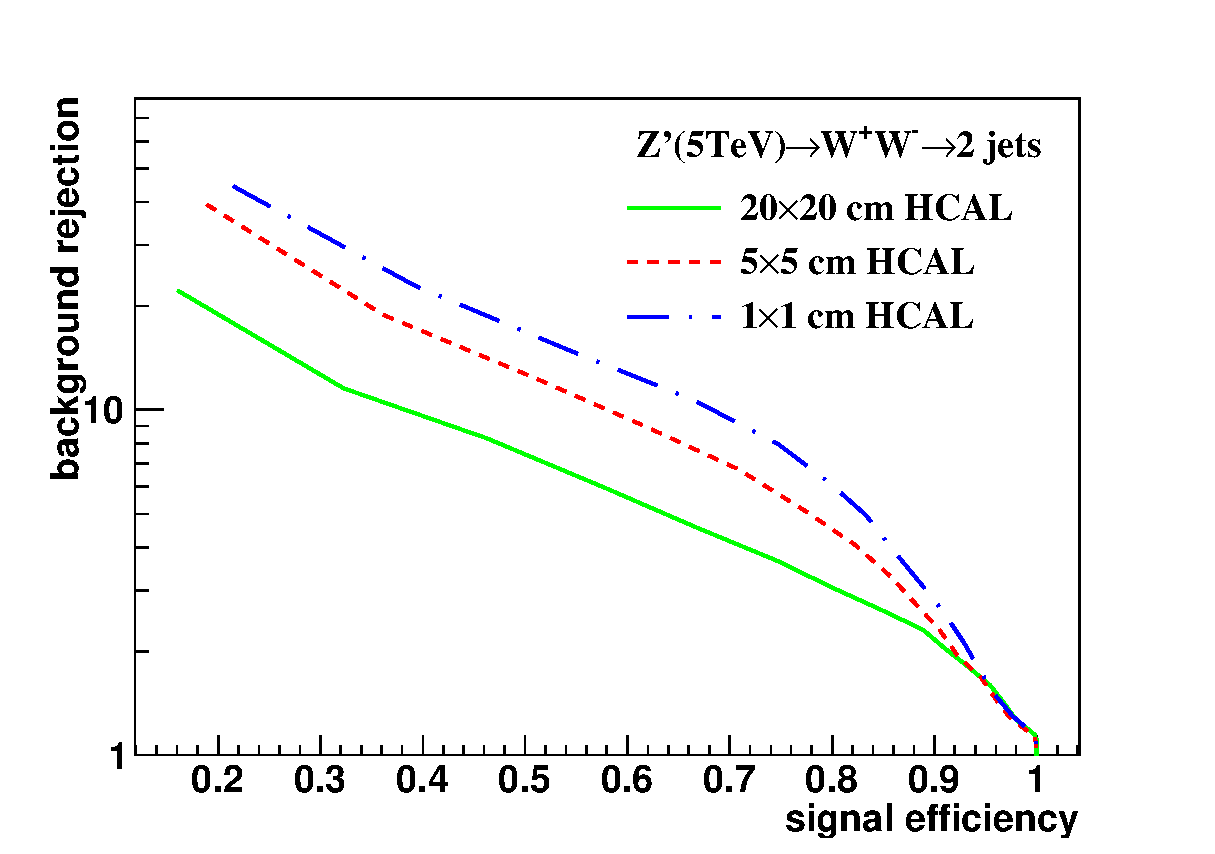
\includegraphics[width=0.43\textwidth]{figs/A_Cluster_mass_mmdt_5tev_eff_1_central_fix_at_Median_bin_ww_qq_log_no_UOF.eps}
  }
  \subfigure[Central at Median($20\times20$=,$5\times5$=,$1\times1$=) change width with cluster at 10TeV] {
  \includegraphics[width=0.43\textwidth]{figs/A_Cluster_mass_mmdt_10tev_eff_1_central_fix_at_Median_bin_ww_qq_log_no_UOF.eps}
  }
 \subfigure[Central at Median($20\times20$=,$5\times5$=,$1\times1$=) change width with cluster at 20TeV] {
 \includegraphics[width=0.43\textwidth]{figs/A_Cluster_mass_mmdt_20tev_eff_1_central_fix_at_Median_bin_ww_qq_log_no_UOF.eps}
 }
 \subfigure[Central at Median($20\times20$=,$5\times5$=,$1\times1$=) change width with cluster at 40TeV] {
 \includegraphics[width=0.43\textwidth]{figs/A_Cluster_mass_mmdt_40tev_eff_1_central_fix_at_Median_bin_ww_qq_log_no_UOF.eps}
 }
\end{center}
\caption{study of "fix central and change width" in mass soft drop at $\beta$=0, signal=ww, with 5, 10, 20, 40TeV c.m. energy and different detector sizes. Cell Size in 20$\times$20, 5$\times$5, and 1$\times$1(cm$\times$cm) are shown in each picture.}
\label{fig:cluster_mass_mmdt_ww_ROC}
\end{figure}


\begin{figure}
\begin{center}
   \subfigure[5TeV at 20$\times$20(cm$\times$cm) with cluster] {
   \includegraphics[width=0.22\textwidth]{figs/Dis_cluster_010_mass_mmdt_tt_5tev_04_tt_no_UOF.eps}
   }
      \subfigure[10TeV at 20$\times$20(cm$\times$cm) with cluster] {
   \includegraphics[width=0.22\textwidth]{figs/Dis_cluster_010_mass_mmdt_tt_10tev_04_tt_no_UOF.eps}
   }
   \subfigure[20TeV at 5$\times$5(cm$\times$cm) with cluster] {
   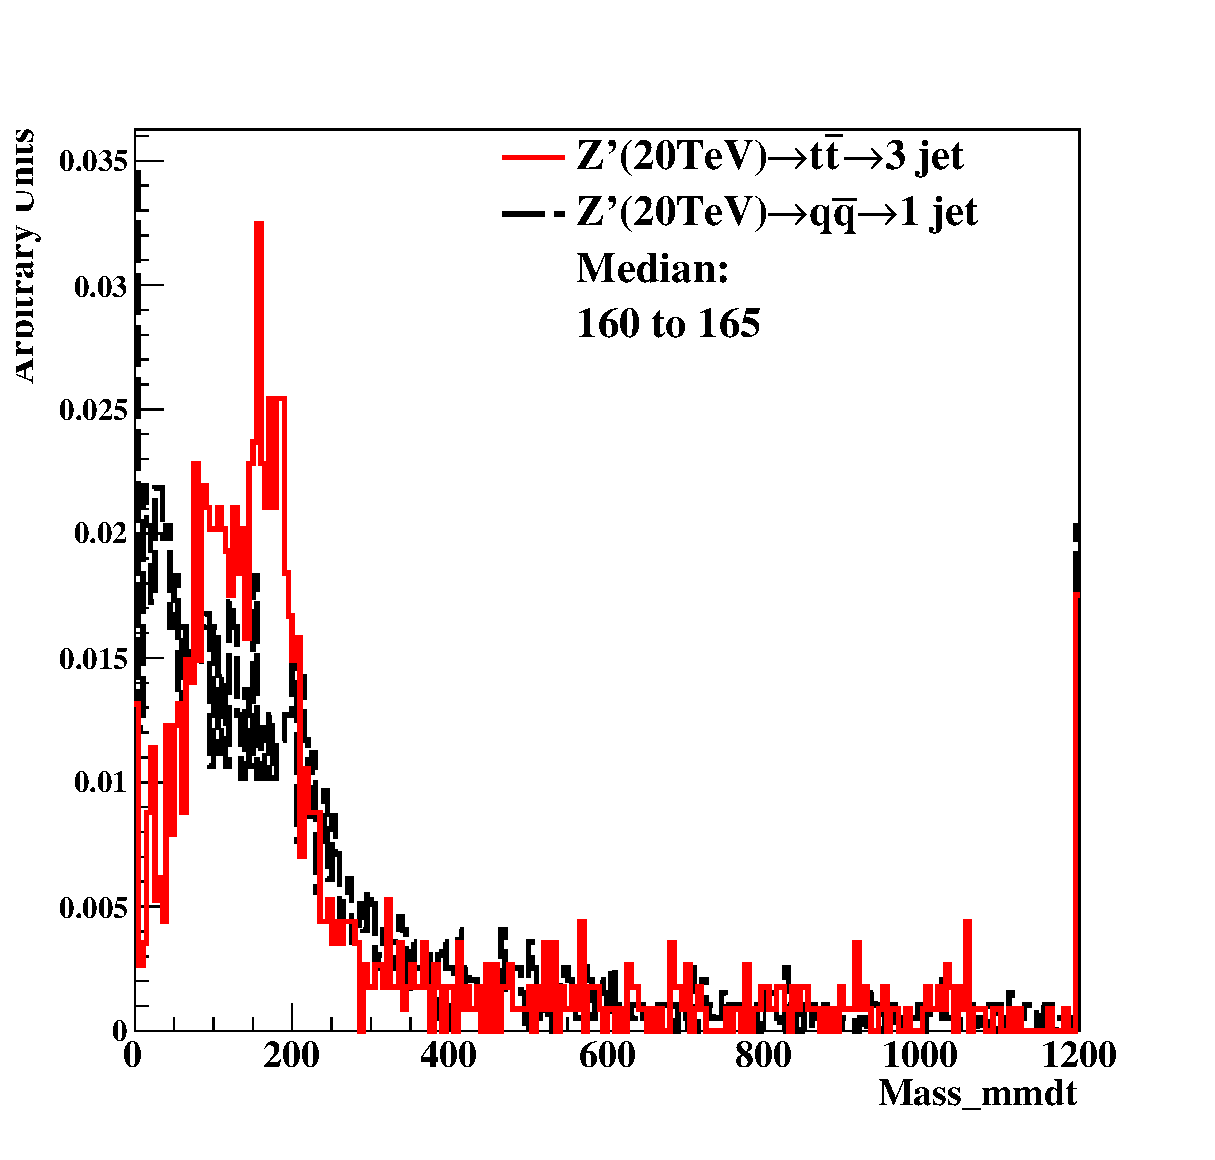
\includegraphics[width=0.22\textwidth]{figs/Dis_cluster_010_mass_mmdt_tt_20tev_04_tt_no_UOF.eps}
   }
    \subfigure[40TeV at 5$\times$5(cm$\times$cm) with cluster] {
   \includegraphics[width=0.22\textwidth]{figs/Dis_cluster_010_mass_mmdt_tt_40tev_04_tt_no_UOF.eps}
   }
   \subfigure[5TeV at 1$\times$1(cm$\times$cm) with cluster] {
   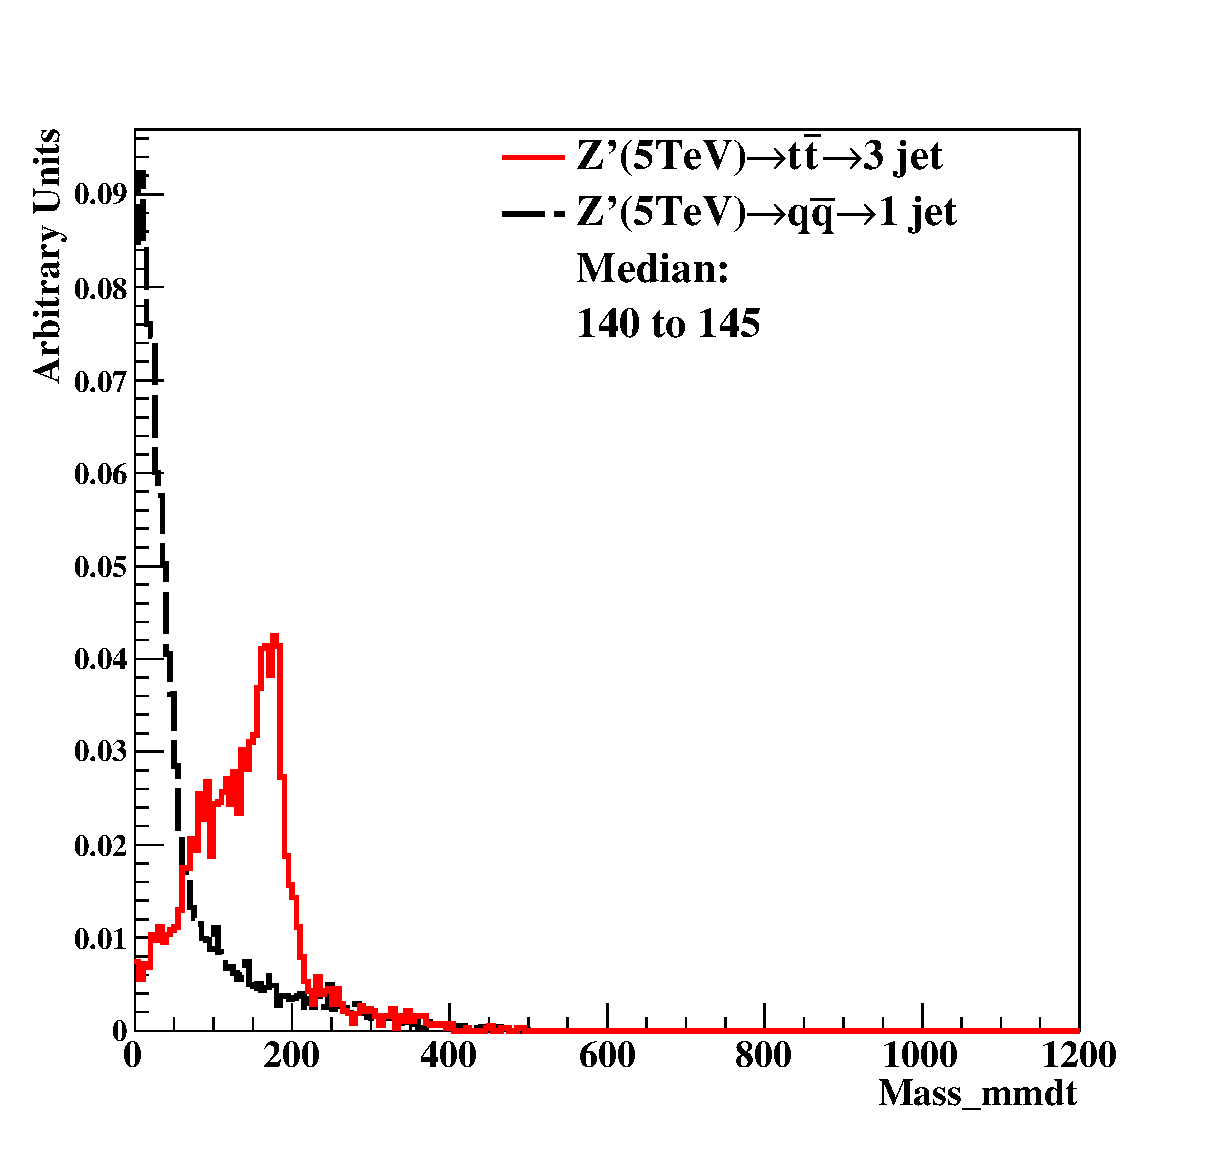
\includegraphics[width=0.22\textwidth]{figs/Dis_cluster_009_mass_mmdt_tt_5tev_04_tt_no_UOF.eps}
   }
   \subfigure[10TeV at 1$\times$1(cm$\times$cm) with cluster] {
   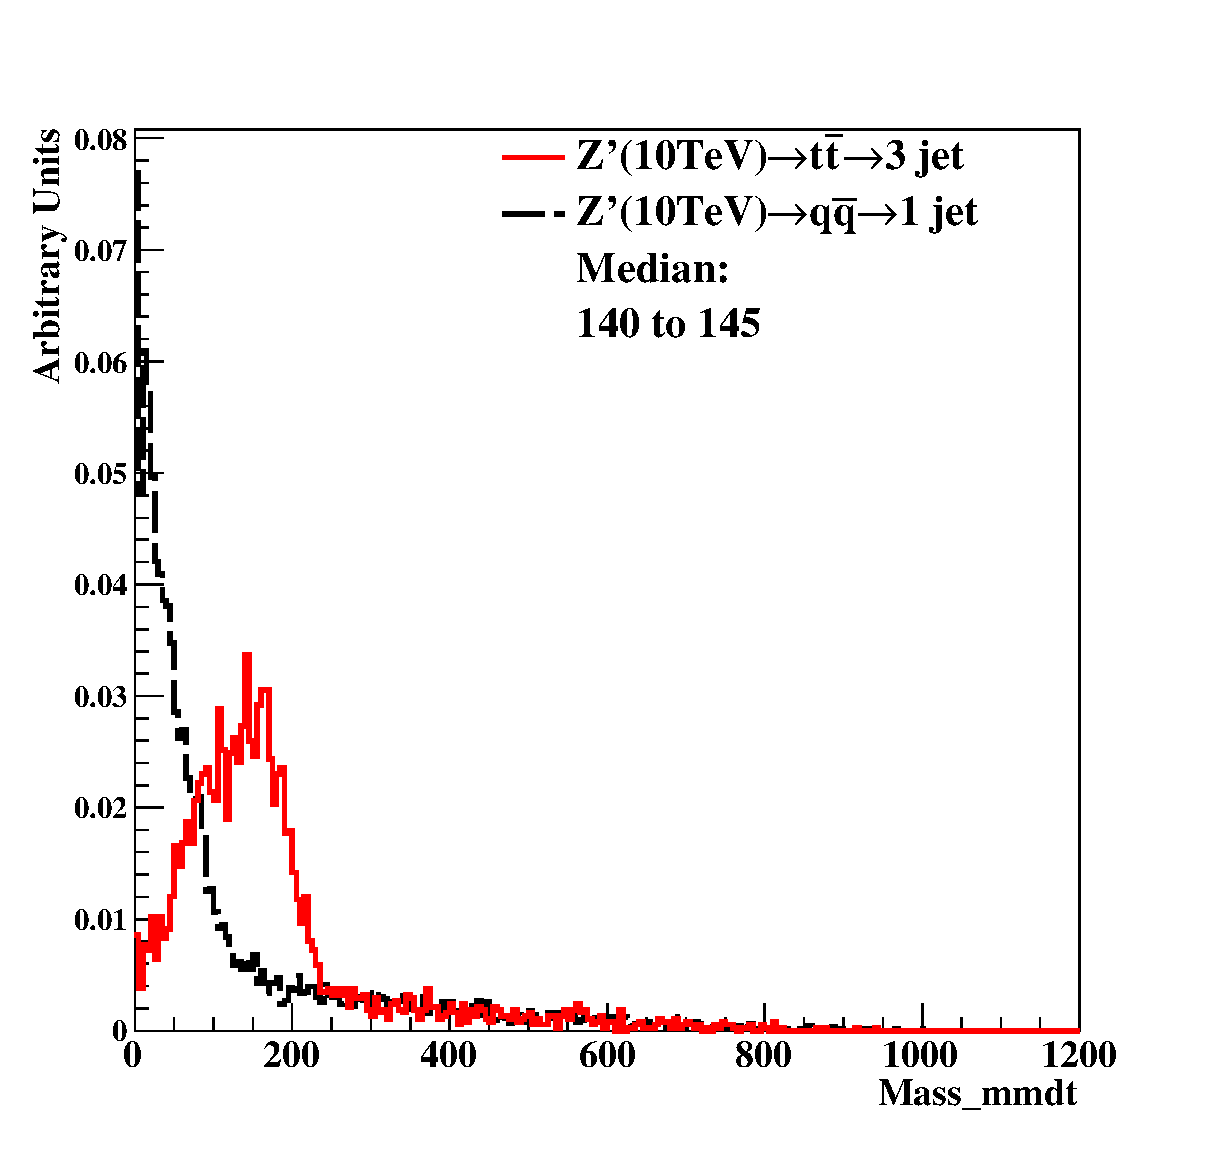
\includegraphics[width=0.22\textwidth]{figs/Dis_cluster_009_mass_mmdt_tt_10tev_04_tt_no_UOF.eps}
   }
   \subfigure[20TeV at 20$\times$20(cm$\times$cm) with cluster] {
   \includegraphics[width=0.22\textwidth]{figs/Dis_cluster_009_mass_mmdt_tt_20tev_04_tt_no_UOF.eps}\hfill
   }
      \subfigure[40TeV at 20$\times$20(cm$\times$cm) with cluster] {
   \includegraphics[width=0.22\textwidth]{figs/Dis_cluster_009_mass_mmdt_tt_40tev_04_tt_no_UOF.eps}\hfill
   }
   \subfigure[5TeV at 5$\times$5(cm$\times$cm) with cluster] {
   \includegraphics[width=0.22\textwidth]{figs/Dis_cluster_012_mass_mmdt_tt_5tev_04_tt_no_UOF.eps}\hfill
   }
    \subfigure[10TeV at 5$\times$5(cm$\times$cm) with cluster] {
   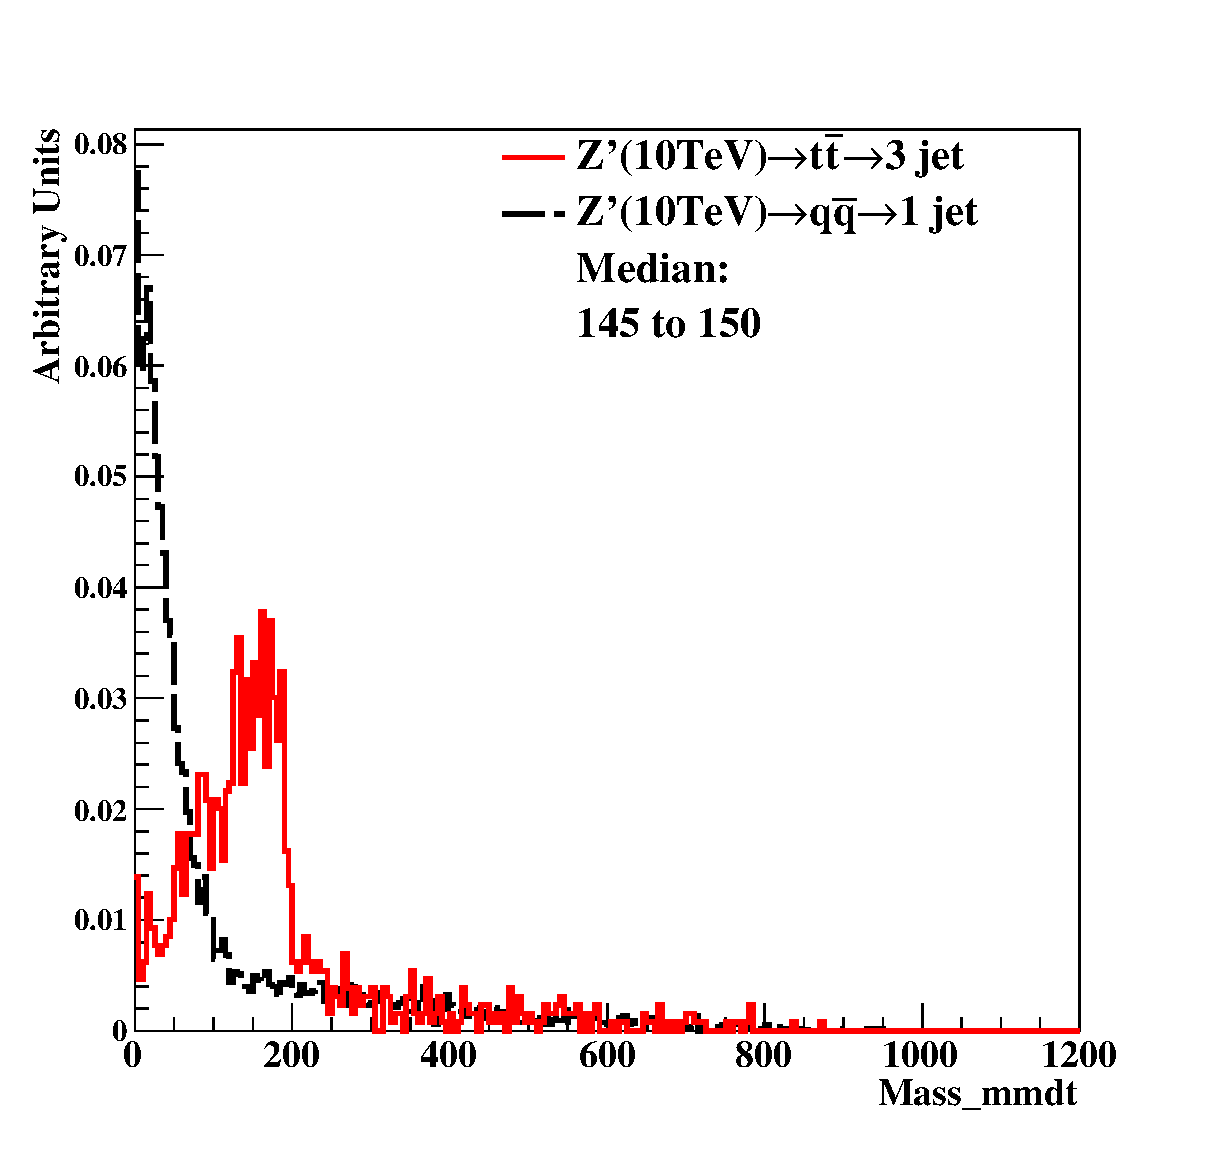
\includegraphics[width=0.22\textwidth]{figs/Dis_cluster_012_mass_mmdt_tt_10tev_04_tt_no_UOF.eps}
   }
   \subfigure[20TeV at 1$\times$1(cm$\times$cm) with cluster] {
   \includegraphics[width=0.22\textwidth]{figs/Dis_cluster_012_mass_mmdt_tt_20tev_04_tt_no_UOF.eps}\hfill
   }
      \subfigure[40TeV at 1$\times$1(cm$\times$cm) with cluster] {
   \includegraphics[width=0.22\textwidth]{figs/Dis_cluster_012_mass_mmdt_tt_40tev_04_tt_no_UOF.eps}
   }
\end{center}
\caption{Distributions of mass soft drop at $\beta$=0, signal=tt, with 5,10,20,40TeV c.m. energy and different detector sizes. Cell Size in 20$\times$20, 5$\times$5, and 1$\times$1(cm$\times$cm) are shown here.}
\label{fig:cluster_mass_mmdt_tt}
\end{figure}


\begin{figure}
\begin{center}
  \subfigure[Central at Median($20\times20$=,$5\times5$=,$1\times1$=) change width with cluster at 5TeV] {
  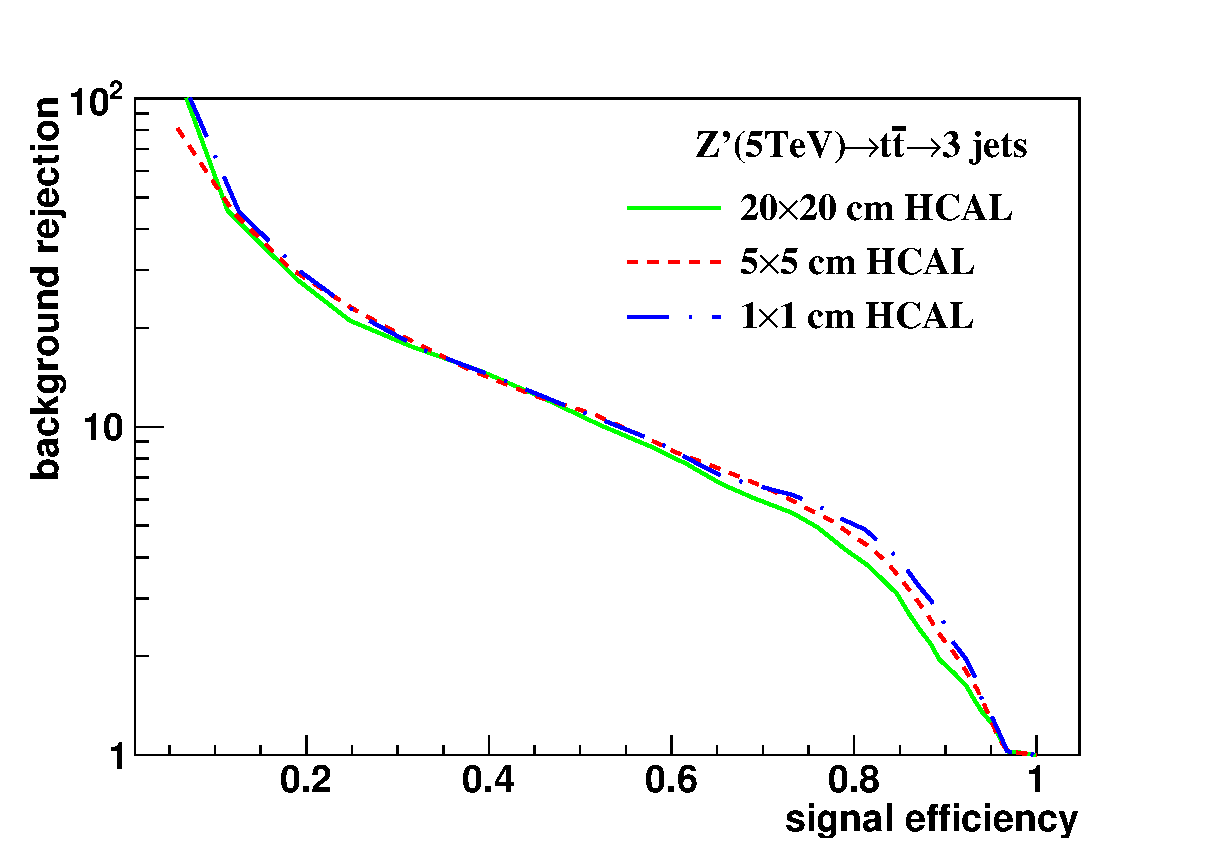
\includegraphics[width=0.43\textwidth]{figs/A_Cluster_mass_mmdt_5tev_eff_1_central_fix_at_Median_bin_tt_qq_log_no_UOF.eps}
  }
  \subfigure[Central at Median($20\times20$=,$5\times5$=,$1\times1$=) change width with cluster at 10TeV] {
  \includegraphics[width=0.43\textwidth]{figs/A_Cluster_mass_mmdt_10tev_eff_1_central_fix_at_Median_bin_tt_qq_log_no_UOF.eps}
  }
 \subfigure[Central at Median($20\times20$=,$5\times5$=,$1\times1$=) change width with cluster at 20TeV] {
 \includegraphics[width=0.43\textwidth]{figs/A_Cluster_mass_mmdt_20tev_eff_1_central_fix_at_Median_bin_tt_qq_log_no_UOF.eps}
 }
 \subfigure[Central at Median($20\times20$=,$5\times5$=,$1\times1$=) change width with cluster at 40TeV] {
 \includegraphics[width=0.43\textwidth]{figs/A_Cluster_mass_mmdt_40tev_eff_1_central_fix_at_Median_bin_tt_qq_log_no_UOF.eps}
 }
\end{center}
\caption{study of "fix central and change width" in mass soft drop at $\beta$=0, signal=tt, with 5, 10, 20, 40TeV c.m. energy and different detector sizes. Cell Size in 20$\times$20, 5$\times$5, and 1$\times$1(cm$\times$cm) are shown in each picture.}
\label{fig:cluster_mass_mmdt_tt_ROC}
\end{figure}



\begin{figure}
\begin{center}
   \subfigure[5TeV at 20$\times$20(cm$\times$cm) with cluster] {
   \includegraphics[width=0.22\textwidth]{figs/Dis_cluster_010_mass_sdb2_ww_5tev_04_800_no_UOF.eps}
   }
      \subfigure[10TeV at 20$\times$20(cm$\times$cm) with cluster] {
   \includegraphics[width=0.22\textwidth]{figs/Dis_cluster_010_mass_sdb2_ww_10tev_04_800_no_UOF.eps}
   }
   \subfigure[20TeV at 20$\times$20(cm$\times$cm) with cluster] {
   \includegraphics[width=0.22\textwidth]{figs/Dis_cluster_010_mass_sdb2_ww_20tev_04_1600_no_UOF.eps}
   }
    \subfigure[40TeV at 20$\times$20(cm$\times$cm) with cluster] {
   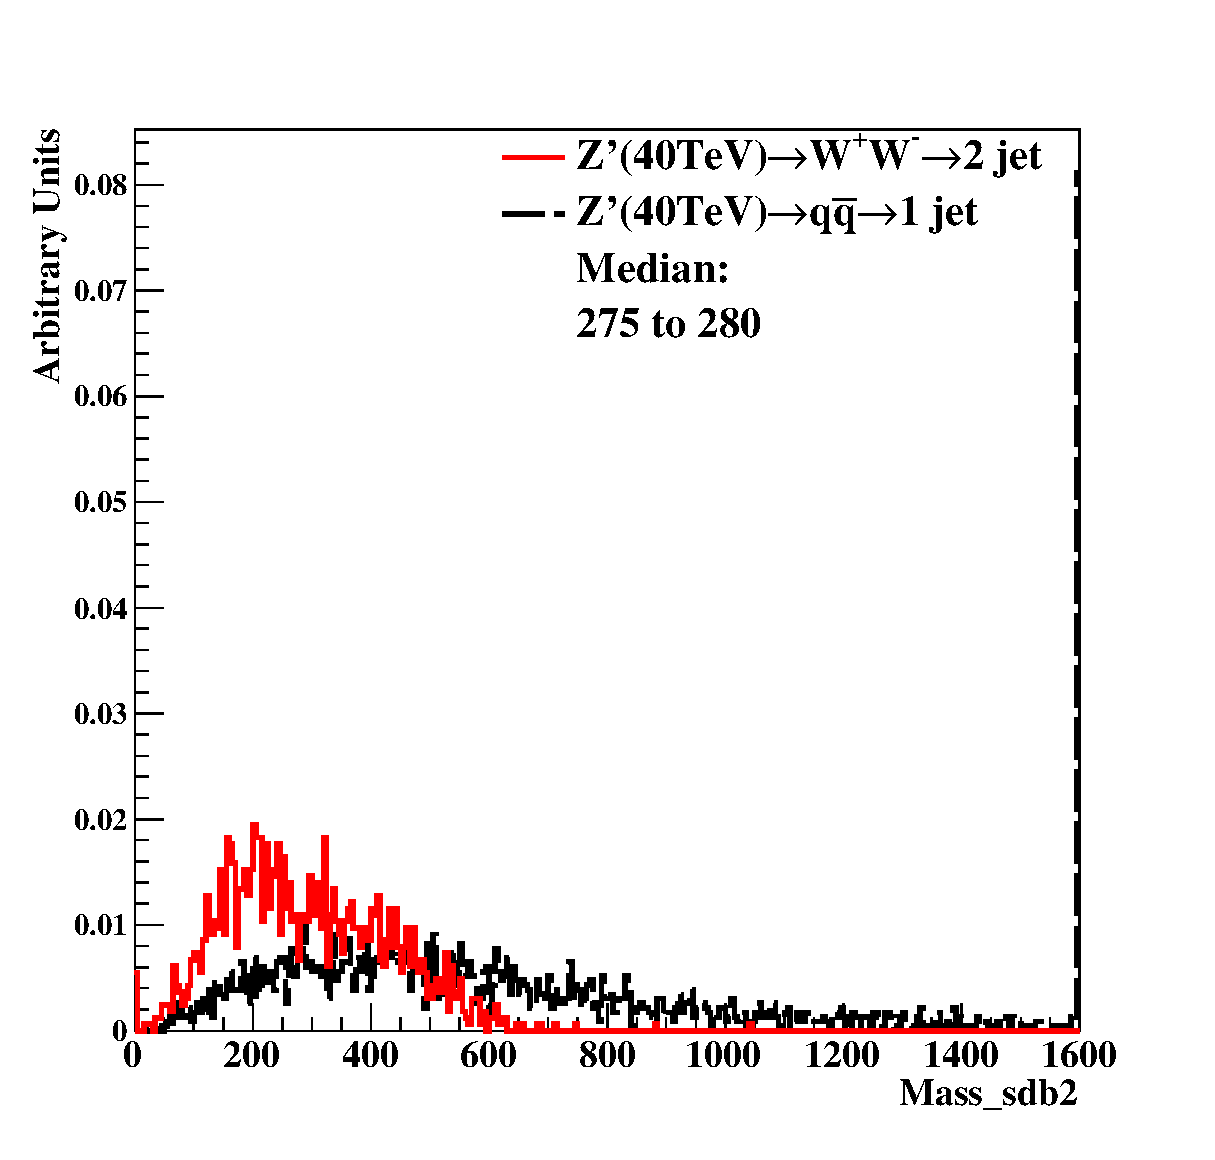
\includegraphics[width=0.22\textwidth]{figs/Dis_cluster_010_mass_sdb2_ww_40tev_04_1600_no_UOF.eps}
   }
   \subfigure[5TeV at 5$\times$5(cm$\times$cm) with cluster] {
   \includegraphics[width=0.22\textwidth]{figs/Dis_cluster_009_mass_sdb2_ww_5tev_04_800_no_UOF.eps}
   }
   \subfigure[10TeV at 5$\times$5(cm$\times$cm) with cluster] {
   \includegraphics[width=0.22\textwidth]{figs/Dis_cluster_009_mass_sdb2_ww_10tev_04_800_no_UOF.eps}
   }
    \subfigure[20TeV at 5$\times$5(cm$\times$cm) with cluster] {
   \includegraphics[width=0.22\textwidth]{figs/Dis_cluster_009_mass_sdb2_ww_20tev_04_1600_no_UOF.eps}\hfill
   }
      \subfigure[40TeV at 5$\times$5(cm$\times$cm) with cluster] {
   \includegraphics[width=0.22\textwidth]{figs/Dis_cluster_009_mass_sdb2_ww_40tev_04_1600_no_UOF.eps}\hfill
   }
   \subfigure[5TeV at 1$\times$1(cm$\times$cm) with cluster] {
   \includegraphics[width=0.22\textwidth]{figs/Dis_cluster_012_mass_sdb2_ww_5tev_04_800_no_UOF.eps}\hfill
   }
    \subfigure[10TeV at 1$\times$1(cm$\times$cm) with cluster] {
   \includegraphics[width=0.22\textwidth]{figs/Dis_cluster_012_mass_sdb2_ww_10tev_04_800_no_UOF.eps}
   }
   \subfigure[20TeV at 1$\times$1(cm$\times$cm) with cluster] {
   \includegraphics[width=0.22\textwidth]{figs/Dis_cluster_012_mass_sdb2_ww_20tev_04_1600_no_UOF.eps}\hfill
   }
      \subfigure[40TeV at 1$\times$1(cm$\times$cm) with cluster] {
   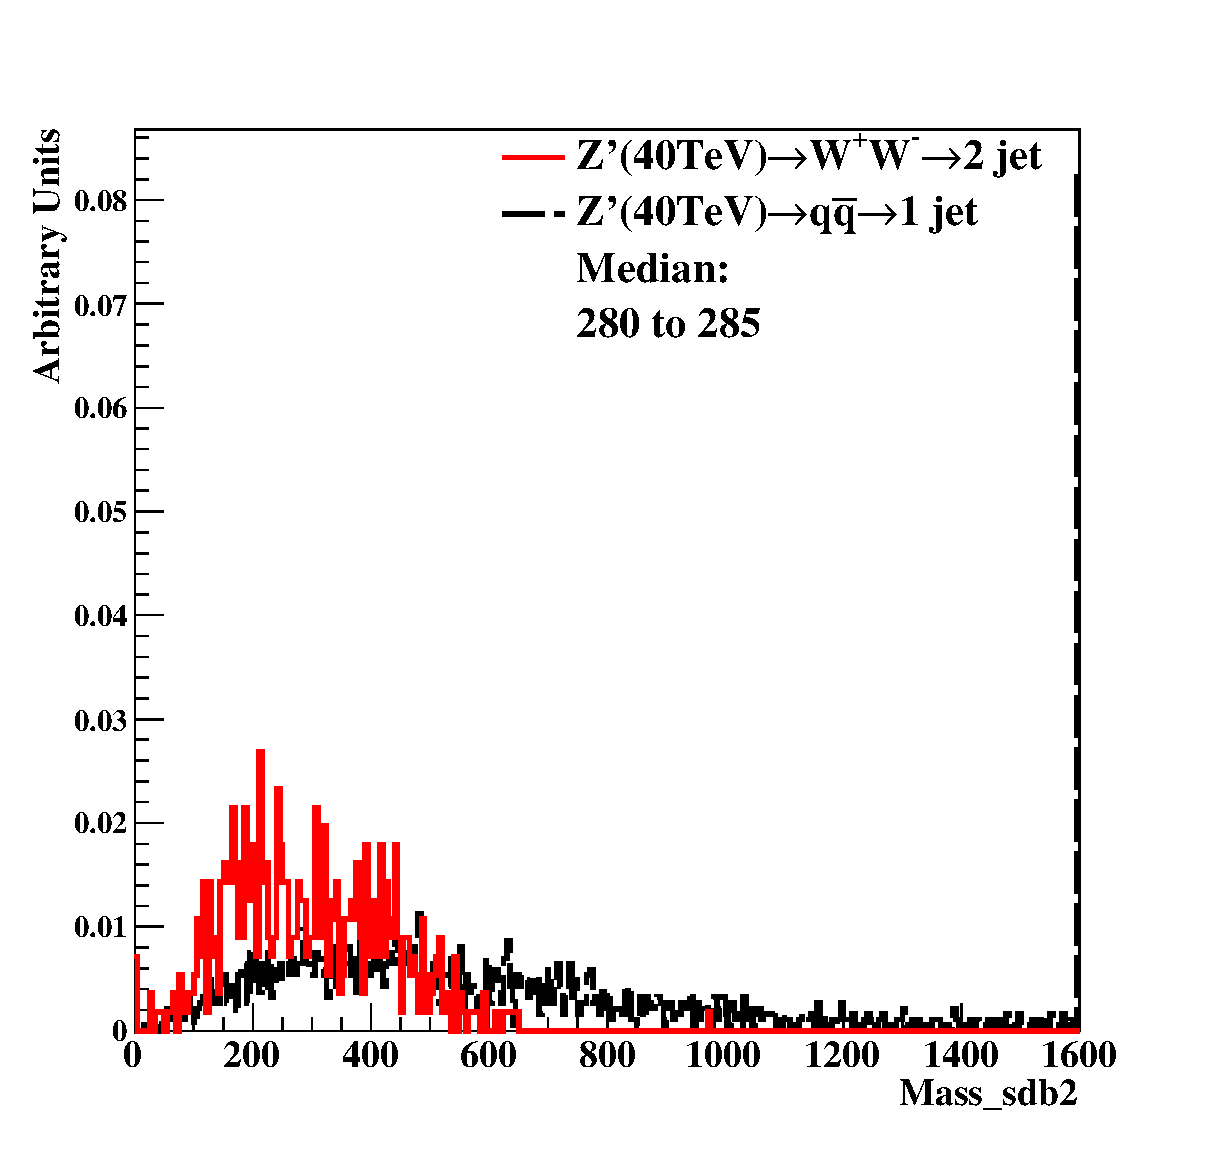
\includegraphics[width=0.22\textwidth]{figs/Dis_cluster_012_mass_sdb2_ww_40tev_04_1600_no_UOF.eps}
   }
\end{center}
\caption{Distributions of mass soft drop at $\beta$=2, signal=ww, with 5,10,20,40TeV c.m. energy  and different detector sizes. Cell Size in 20$\times$20, 5$\times$5, and 1$\times$1(cm$\times$cm) are shown here.}
\label{fig:cluster_mass_sdb2_ww}
\end{figure}


\begin{figure}
\begin{center}
  \subfigure[Central at Median($20\times20$=,$5\times5$=,$1\times1$=) change width with cluster at 5TeV] {
  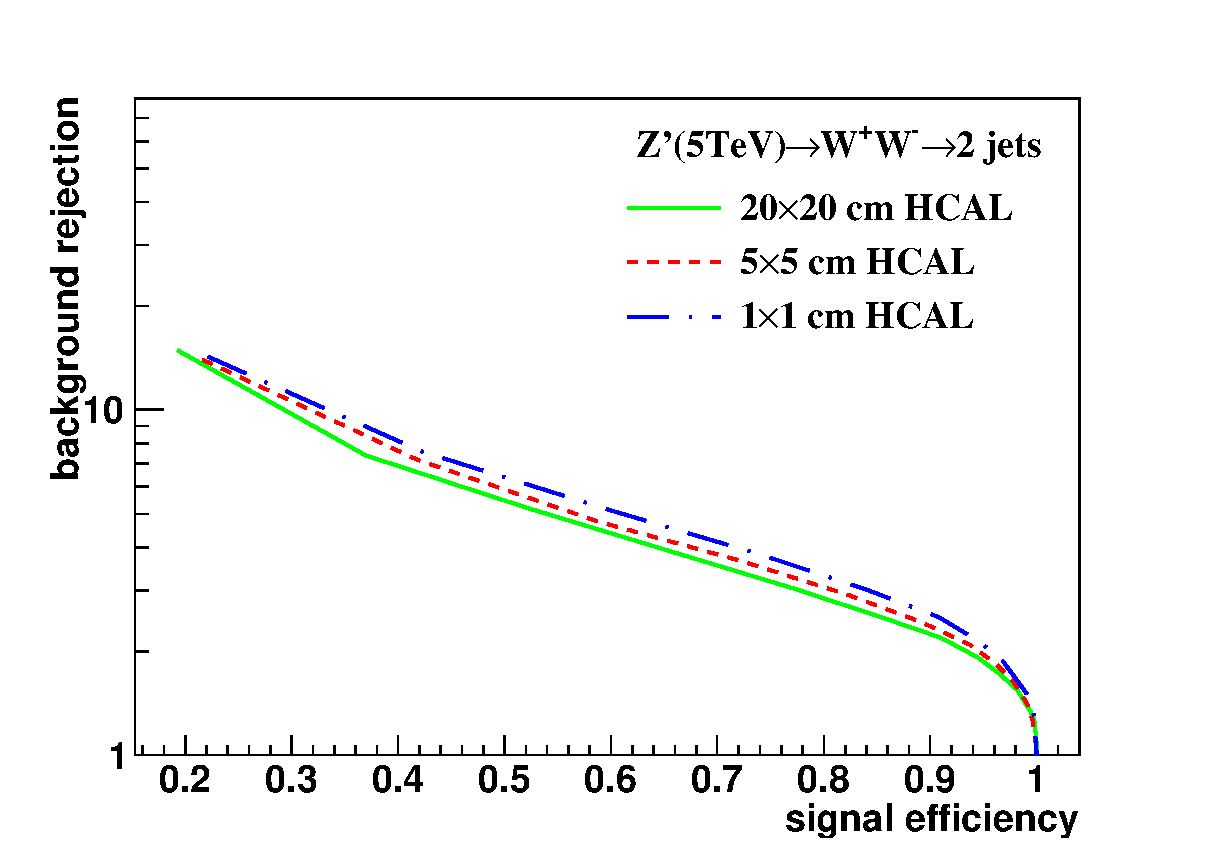
\includegraphics[width=0.43\textwidth]{figs/A_Cluster_mass_sdb2_5tev_eff_1_central_fix_at_Median_bin_ww_qq_log_no_UOF.eps}
  }
  \subfigure[Central at Median($20\times20$=,$5\times5$=,$1\times1$=) change width with cluster at 10TeV] {
  \includegraphics[width=0.43\textwidth]{figs/A_Cluster_mass_sdb2_10tev_eff_1_central_fix_at_Median_bin_ww_qq_log_no_UOF.eps}
  }
 \subfigure[Central at Median($20\times20$=,$5\times5$=,$1\times1$=) change width with cluster at 20TeV] {
 \includegraphics[width=0.43\textwidth]{figs/A_Cluster_mass_sdb2_20tev_eff_1_central_fix_at_Median_bin_ww_qq_log_no_UOF.eps}
 }
 \subfigure[Central at Median($20\times20$=,$5\times5$=,$1\times1$=) change width with cluster at 40TeV] {
 \includegraphics[width=0.43\textwidth]{figs/A_Cluster_mass_sdb2_40tev_eff_1_central_fix_at_Median_bin_ww_qq_log_no_UOF.eps}
 }
\end{center}
\caption{study of "fix central and change width" in mass soft drop at $\beta$=2, signal=ww, with 5, 10, 20, 40TeV c.m. energy and different detector sizes. Cell Size in 20$\times$20, 5$\times$5, and 1$\times$1(cm$\times$cm) are shown in each picture.}
\label{fig:cluster_mass_sdb2_ww_ROC}
\end{figure}


\begin{figure}
\begin{center}
   \subfigure[5TeV at 20$\times$20(cm$\times$cm) with cluster] {
   \includegraphics[width=0.22\textwidth]{figs/Dis_cluster_012_mass_sdb2_tt_5tev_04_tt_1200_no_UOF.eps}
   }
      \subfigure[10TeV at 20$\times$20(cm$\times$cm) with cluster] {
   \includegraphics[width=0.22\textwidth]{figs/Dis_cluster_010_mass_sdb2_tt_10tev_04_tt_1200_no_UOF.eps}
   }
   \subfigure[20TeV at 20$\times$20(cm$\times$cm) with cluster] {
   \includegraphics[width=0.22\textwidth]{figs/Dis_cluster_010_mass_sdb2_tt_20tev_04_tt_2400_no_UOF.eps}
   }
    \subfigure[40TeV at 20$\times$20(cm$\times$cm) with cluster] {
   \includegraphics[width=0.22\textwidth]{figs/Dis_cluster_010_mass_sdb2_tt_40tev_04_tt_2400_no_UOF.eps}
   }
   \subfigure[5TeV at 5$\times$5(cm$\times$cm) with cluster] {
   \includegraphics[width=0.22\textwidth]{figs/Dis_cluster_009_mass_sdb2_tt_5tev_04_tt_1200_no_UOF.eps}
   }
   \subfigure[10TeV at 5$\times$5(cm$\times$cm) with cluster] {
   \includegraphics[width=0.22\textwidth]{figs/Dis_cluster_009_mass_sdb2_tt_10tev_04_tt_1200_no_UOF.eps}
   }
   \subfigure[20TeV at 5$\times$5(cm$\times$cm) with cluster] {
   \includegraphics[width=0.22\textwidth]{figs/Dis_cluster_009_mass_sdb2_tt_20tev_04_tt_2400_no_UOF.eps}\hfill
   }
      \subfigure[40TeV at 5$\times$5(cm$\times$cm) with cluster] {
   \includegraphics[width=0.22\textwidth]{figs/Dis_cluster_009_mass_sdb2_tt_40tev_04_tt_2400_no_UOF.eps}\hfill
   }
   \subfigure[5TeV at 1$\times$1(cm$\times$cm) with cluster] {
   \includegraphics[width=0.22\textwidth]{figs/Dis_cluster_012_mass_sdb2_tt_5tev_04_tt_1200_no_UOF.eps}\hfill
   }
    \subfigure[10TeV at 1$\times$1(cm$\times$cm) with cluster] {
   \includegraphics[width=0.22\textwidth]{figs/Dis_cluster_012_mass_sdb2_tt_10tev_04_tt_1200_no_UOF.eps}
   }
   \subfigure[20TeV at 1$\times$1(cm$\times$cm) with cluster] {
   \includegraphics[width=0.22\textwidth]{figs/Dis_cluster_012_mass_sdb2_tt_20tev_04_tt_2400_no_UOF.eps}\hfill
   }
      \subfigure[40TeV at 1$\times$1(cm$\times$cm) with cluster] {
   \includegraphics[width=0.22\textwidth]{figs/Dis_cluster_012_mass_sdb2_tt_40tev_04_tt_2400_no_UOF.eps}
   }
\end{center}
\caption{Distributions of mass soft drop at $\beta$=2, signal=tt, with 5,10,20,40TeV c.m. energy and different detector sizes. Cell Size in 20$\times$20, 5$\times$5, and 1$\times$1(cm$\times$cm) are shown here.}
\label{fig:cluster_mass_sdb2_tt}
\end{figure}


\begin{figure}
\begin{center}
  \subfigure[Central at Median($20\times20$=,$5\times5$=,$1\times1$=) change width with cluster at 5TeV] {
  \includegraphics[width=0.43\textwidth]{figs/A_Cluster_mass_sdb2_5tev_eff_1_central_fix_at_Median_bin_tt_qq_log_no_UOF.eps}
  }
  \subfigure[Central at Median($20\times20$=,$5\times5$=,$1\times1$=) change width with cluster at 10TeV] {
  \includegraphics[width=0.43\textwidth]{figs/A_Cluster_mass_sdb2_10tev_eff_1_central_fix_at_Median_bin_tt_qq_log_no_UOF.eps}
  }
 \subfigure[Central at Median($20\times20$=,$5\times5$=,$1\times1$=) change width with cluster at 20TeV] {
 \includegraphics[width=0.43\textwidth]{figs/A_Cluster_mass_sdb2_20tev_eff_1_central_fix_at_Median_bin_tt_qq_log_no_UOF.eps}
 }
 \subfigure[Central at Median($20\times20$=,$5\times5$=,$1\times1$=) change width with cluster at 40TeV] {
 \includegraphics[width=0.43\textwidth]{figs/A_Cluster_mass_sdb2_40tev_eff_1_central_fix_at_Median_bin_tt_qq_log_no_UOF.eps}
 }
\end{center}
\caption{study of "fix central and change width" in mass soft drop at $\beta$=2, signal=tt, with 5, 10, 20, 40TeV c.m. energy and different detector sizes. Cell Size in 20$\times$20, 5$\times$5, and 1$\times$1(cm$\times$cm) are shown in each picture.}
\label{fig:cluster_mass_sdb2_tt_ROC}
\end{figure}





